% !TEX root = ../master.tex
\chapter{Design and Methodology}
\label{chap:design}
This chapter describes which research method is used to design a solution 
that answers the initial questions posed in the first chapter.
The considerations that contribute to the design of this solution are outlined 
and form the foundation for its implementation in the next chapter.

\section{Employed Methodology}

Preceding to the practical part of this thesis, 
the method to follow along shall be laid out here.
One suitable method is the general concept of \emph{design science research}, also known as \emph{constructive research}, 
since it involves the development and evaluation of artifacts to solve domain specific problems.
It therefore conveys a improved practical relevance in comparison to purely descriptive research methods,
while the outcomes still create scientific knowledge
\autocite[][p.~v]{dresh2015designresearch}.
The conducted research must design an artifact, such as a construct, model or method, that solves a relevant problem in a specific field, which is evaluated regarding its utility, quality and efficacy.
The performed research should be based on rigorous scientific methods and contribute to the current theoretical body of knowledge.
The conducted design process must take into account the practical environment it is executed in and use the available resources.
A conclusion of the project for both technology-oriented as well as management-oriented audiences should be presented in the end
\autocite[][p.~70]{dresh2015designresearch}.

\begin{figure}[hbt]
	\centering
	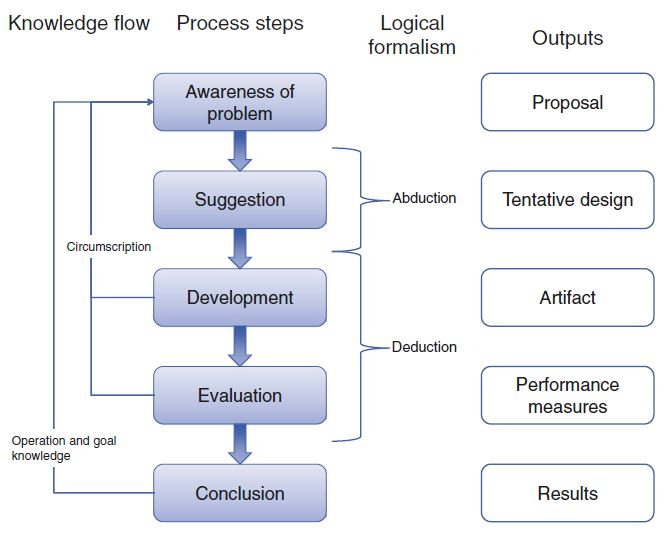
\includegraphics[width=0.8\textwidth, keepaspectratio]{resources/designscienceresearchoutputs.jpg}
	\caption{\label{fig:design:designscience} Process steps and outputs of design science research. Reprinted from \textcite[][p.~83]{dresh2015designresearch}}
\end{figure}

Figure \ref{fig:design:designscience} displays the steps that are found in the process of design science research. 
Those are the steps that guide the execution of this thesis.
The awareness and relevance for the given problem has already been given in section \vref{sec:into:context}.
Looking back to the original research questions (see section \vref{sec:intro:goals}) two focuses have been identified for this thesis:

\begin{itemize}
    \item Which computer vision techniques can be used to detect persons and objects within an elevator car and in front of the lift and estimate their spacial volume?
    \item How can the information acquired by a system that uses such methods constitute to the optimization of algorithms that control the movement plan for elevators?
\end{itemize}


To answer the two questions, the conducted research is therefore twofold.
The first part involves the design and experimental implementation of a system to gather passengers volume data in elevators.
The second part deals with the integration of this information into a scheduling algorithm.
Outlined below are the steps that are taken to
suggest a tentative design for each, develop the artifacts and evaluate them.

For the  design and implementation of a vision system to gather volume data of passengers,
the following steps are performed:

\begin{enumerate}
    \item Find a typical or actual elevator control system architecture and define the positions to integrate the necessary components for an vision system into it.
    \item Define the exact type and structure of the information that the vision system should be able to detect.
    \item Find an algorithmic approach to  passenger detection and volume estimation that is suitable to generate the required data.
    \item Match the approach with an possible hardware setup to perform tests with it.
    \item Test the proposed detection system in an real world experiment that includes  exemplary footage from within an cabin and of a lobby.
    \item Evaluate the results of the test for the functionality and effectiveness of the employed system.
\end{enumerate}

For the integration of the  passenger data into existing scheduling algorithm the following steps are performed:

\begin{enumerate}
    \item Define a suitable elevator configuration that could possibly benefit from the information that the vision system can provide. 
    Find a typical or actual control algorithm that is used for such a configuration.
    \item Adapt the scheduling algorithm to use the additional information.
    \item Compare the two versions of the algorithm in order to determine their effectiveness regarding a suitable metric.
    A simulation is used to perform this comparison.
\end{enumerate}

%\begin{figure}[hbt]
%	\centering
%	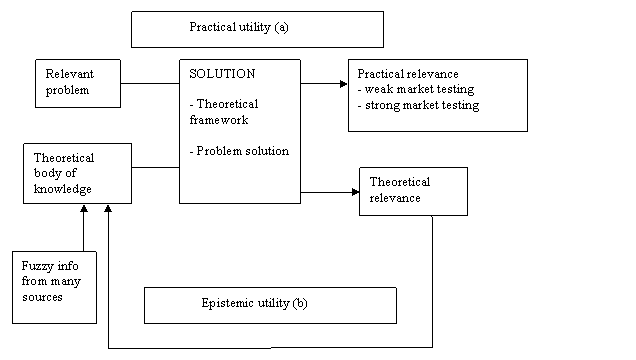
\includegraphics[width=1.0\textwidth, keepaspectratio]{resources/Rasvan_constructive_research_diagram}
%	\caption{\label{fig:design:constructiveresearch} Elements of constructive research. Source:
%	\url{https://en.wikipedia.org/wiki/File:Rasvan_constructive_research_diagram.gif}}
%\end{figure}
 
\section{Visual System}
TODO
\subsection{Proposal for Integration into Elevator Control System Architecture}
TODO
for hardware setup
- no additional sensory
- add cv system (computer) and multiple cams inside each cabin
- add cv system (computer) and multiple or one cam outside on each floor
\subsection{Output Data Definition}
TODO
- for each objects weather it is a person or an cargo object
- for each persons a volume description approximated by an inner and outer ellipse (or simple: circle) as the ground area and a height
- for the cargo objects an approximation as a ground area and a height, possible area types: convex hull most outer circumfence projected to the ground OR estimation by surrounding rectangle
- total number of passengers and cargo objects inside and in-front
\subsection{Detection Technique}
TODO
\subsection{Test Arrangement and Validation Strategy}
TODO

\section{Scheduling Algorithm}
TODO
\subsection{Suitable Elevator Configuration}
Since the camera system is suitable to detect passengers as well as cargo objects,
it seems reasonable to apply the passenger information 
to a scheduling algorithm of an elevator system which conveys both of them.
Looking back at the categorization of elevators, cargo lifts meet this specification.
Typically 



TODO
- a greater impact could be expected when there is a mixture in traffic including both persons and cargo objects such. 
- looking back at the categorization of elevators a cargo lift that also conveys people would fulfill this
- imaginable real world scenarios: hospital where also patient beds are moved (which should have an empty elevator and be prioritized) OR multistory storage buildings where also people use it OR auxiliary lifts in office buildings that carry the janitor cars and other cargo regularly (typically only lift available)
- standard collective control or sequential control
\subsection{Adaption of Scheduling Algorithm}
TODO
- when no large cargo is there: collective control
- when large cargo is there: sequential control
- consideration: what to do to switch between collective and seqential control?
\subsection{Preparation for Simulation and Validation Strategy}

TODO simulation configuration:
\autocite[][p.~347]{barney2016handbook}

\begin{table}[]
\centering
\begin{tabular}{lrl}
\textbf{Description} \hspace{5cm}   & \multicolumn{1}{l}{\textbf{Value}}   & \textbf{Unit}   \\
\hline
\multicolumn{3}{l}{\textbf{Building data}} \\
Number of floors & 8 &        \\
Interfloor distances & 3.5 & $m$\\
%& & \\
\hline
\multicolumn{3}{l}{\textbf{Lift data}}     \\
Number of lifts & 1 & \\
Rated weight load & 5000 & $kg$\\
Rated passenger capacity & 65 & \\
Rated Speed & 1.6 & $ms^{-1}$ \\
Door opening time & 1.5 & $s$\\
Door closing time & 1.5 & $s$\\
Flight time single floor & 8 & $s$\\
%& & \\
\hline
\multicolumn{3}{l}{\textbf{Passenger Data}}\\
Arrival rates for floors & TODO & $ \mathbb{N} \times s \rightarrow s^{-1}$\\
Weight an volume distribution & see below & $kg \times m \times m \times m \rightarrow \mathbb{R}$\\
%Volume distribution & see below  & $m \times m \times m \rightarrow \mathbb{R} $\\
Transfer time into / out of car & 2 & $s$\\
Floor bias & unbiased & $ \mathbb{N} \times \mathbb{N} \rightarrow \mathbb{R} $ \\
%& & \\
\hline
\multicolumn{3}{l}{\textbf{Cargo Data}}\\
Arrival rates for floors & TODO & $\mathbb{N} \times s \rightarrow s^{-1}$\\
Weight an volume distribution & see below & $kg \times m \times m \times m \rightarrow \mathbb{R}$\\
%Volume distribution & see below  & $m \times m \times m \rightarrow \mathbb{R} $\\
Transfer time into / out of car & 5 & $s$\\
Floor bias & unbiased & $ \mathbb{N} \times \mathbb{N} \rightarrow \mathbb{R} $ \\
%& & \\
\hline
\multicolumn{3}{l}{\textbf{Simulation Parameters}}\\
Simulation Period & 1 & $h$\\
Time slice & 0.1 & $s$\\
Number of simulations & 100 & \\
\end{tabular}
\caption{\label{tab:design:simulationconfig} General configuration for the comparative simulation}
\end{table}

data from eg. \url{https://www.kone.de/aufzug-aufzuege.aspx} \url{https://www.kone.de/neubau/aufzug-aufzuege/lastenaufzug-bettenaufzug-transys/}
and also \autocite[][p.~349]{barney2016handbook}

which data to use: \autocite[][p.~347]{barney2016handbook}

TODO
TODO define measurements to take
 

%\section{Requirements}
%TODO
%\autocite[][]{xang2016trafficlist} has done tehe same and patentet it :(
%\section{Conduction of Method}
%TODO the method determines which steps to take
%TODO, choose possible approach from sota
%\section{Proposed Solution}
%TODO next two are included?
%\section{Architectural Plan}
%TODO necessary? yes
%\section{Algorithmic Approach}
%TODO necessary? yes
%\section{Validation Strategy}
%TODO
